\chapter{LibChain}
LibChain should allows to create contracts between publisher and libraries that differ from the classical subscription models for digital media. 


\section{Architecture Overview}
The main architecture of LibChain is divided into three parts: React that is used to implement a prototypical library page, NodeJs that provides a REST interface that enables the connection to the frontend and the ethereum blockchain where the LibChain contracts are deployed on. Communication between the NodeJs backend and the blockchain are realized through the \texttt{Web3.js} api.

\vspace{0.3cm}
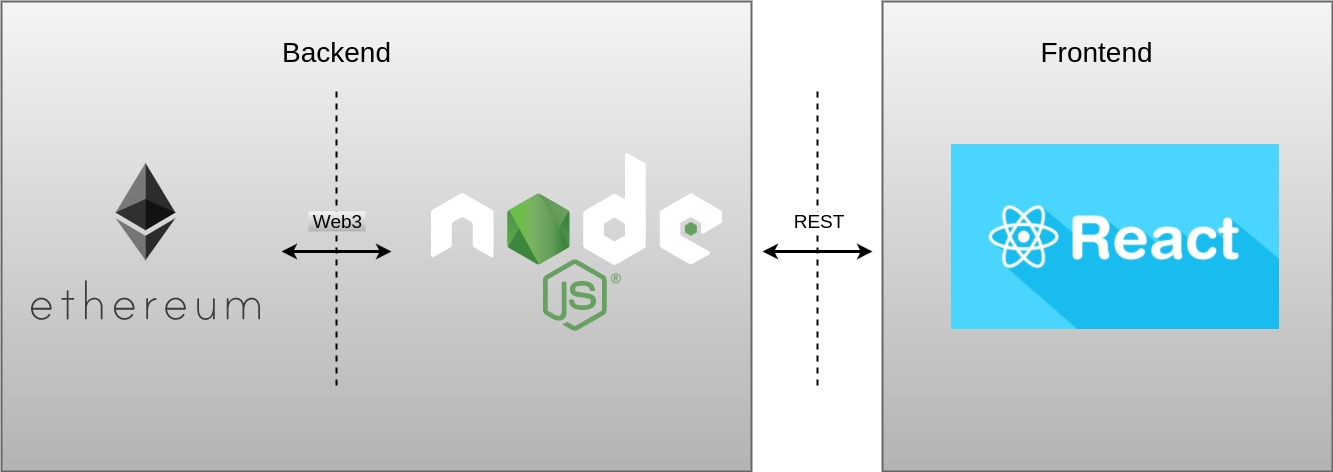
\includegraphics[width=\textwidth]{architecture.jpg}
\subsection{Backend}


\subsection{Frontend}


\section{Smart Contracts}
LibChain implements smart contracts for publisher, libraries and books that provides functionality to publish, buy and lend books in the LibChain ecosystem. 


\vspace{0.3cm}
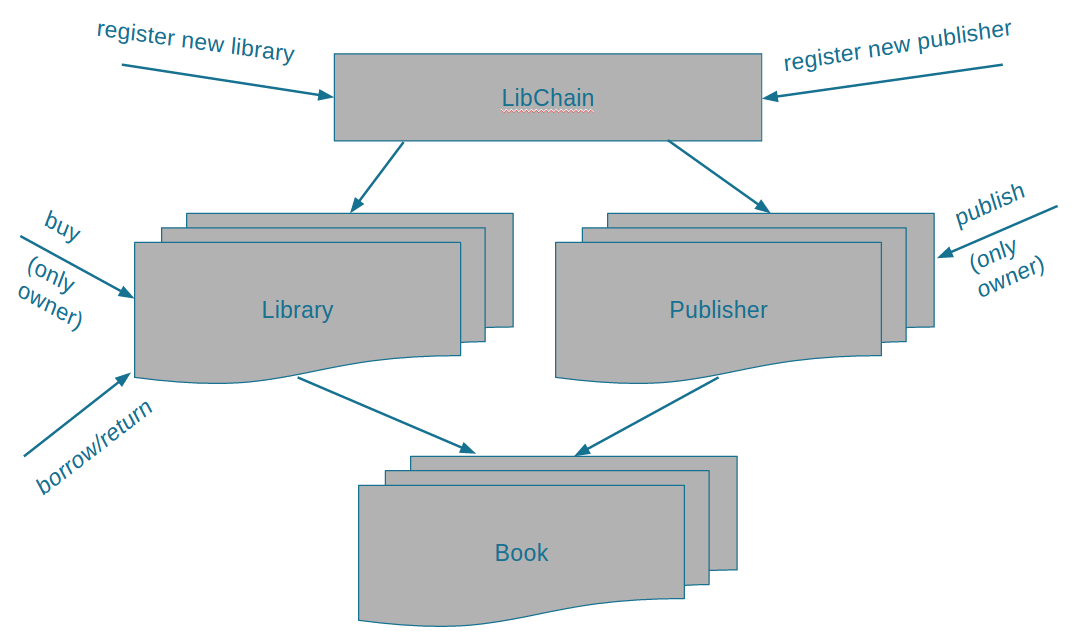
\includegraphics[width=\textwidth]{contracts.png}

\subsection{LibChain}
The LibChain contract is used to instantiate new libraries and publisher. It also provides getters for retrieving existent instances.

\subsection{Book}
The Book contract collects meta-informations like title and year of publication. It also has a field \textit{gateway} that defines the access point to the digital media (for example a link to the publishers book repository). It also contains the publisher address where an instance could be bought. Furthermore it contains some variables to get books statistics, e.g. the amount of sold instances or loans.


\begin{lstlisting}
contract Book {

	address public _owner;
	string public _publisher;
	uint public _year;
	string public _gateway;
	string public _isbn;
	
	mapping (address => uint) public _balances;
	uint sumOfSoldInstances;
	uint sumOfLoans;
  
	function Book(string pub, uint year, string id, string gate) {
  	_owner = msg.sender;
		_publisher = pub;
		_year = year;
		_gateway = gate;
		_isbn = id;
	}


	function getBookInfo() constant returns (uint, string, string, 		string, uint, address, address) 
	{
	 	return (_year, _isbn, _gateway, _publisher, 	_balances[msg.sender], _owner, this);
	}

	function buy(address buyer, uint amount) {
		_balances[buyer] += amount;
		sumOfSoldInstances++;
	}

}
\end{lstlisting}

\subsection{Publisher}
The publisher contract allows to instantiate new books and add them to the publishers catalogue. It's primary used to publish books and sell instances to libraries.

\begin{lstlisting}
function publishBook(uint year, string id, string gate) returns(address bookContract){
		publishedBooks.push(new Book(name, year, id, gate));
		sumOfPublications++;
		(..)
		return publishedBooks[bookNum-1];
	}
\end{lstlisting}

As a Book is a smart contract, it get's a unique address. Therefore, a library is able to call the \texttt{buyBook}-function to get the ownership of permanent instances.

\begin{lstlisting}
	function buyBook(address bookContract, uint amount) constant {
		Book book = Book(bookContract);
		book.buy(msg.sender, amount);	
		bills[msg.sender][bookContract] += amount;

		sumOfSoldInstances += amount;
	}
\end{lstlisting}

\subsection{Library}
The library contract contains functions to buy book instances from publisher contracts and to perfom borrow and return requests.

\paragraph*{buy}
On a buy call, the publishers buy function is called to make a note for this purchase on the publishers site. This information could be used to pay the bill in the real world.
Then the book with the requested amount of instances is stored in the libraries inventory and makes the lending possible to the library users ( see the borrow function ).

\begin{lstlisting}
	function buy(address bookContract, address publisherContract, uint amount) returns (bool) {
		Publisher pub = Publisher(publisherContract);
		pub.buyBook(bookContract, amount);
        Book book = Book(bookContract);
        if(inventory[book].amount == 0){
            inventory[book] = BookMeta(book, amount, amount);
		    _libBooks.push(book);
		} else {
            inventory[book].amount += amount;
            inventory[book].availableInstances += amount;
		}

		sumOfBoughtInstances += amount;
		return true;
	}
\end{lstlisting}


\paragraph*{borrow \label{sssec:contractborrow}}
For borrowing books, it's first check whether an instance is currently available. In addition it's ensured that a user can only borrow one instance of a book at once.

Then, the users public key is stored to the book object in the inventory. The public key is used for checking the access authorization of the user (see hasAccessToInstance function).

\begin{lstlisting}
function borrow(address bookContract, string publicKey, string userId) returns (bool) {

		if(inventory[bookContract].availableInstances <= 0) return false;

		//check if this book already loaned to user
        if (sha3(users[userId].pubkeys[bookContract]) != sha3("")){
            return false;
        }


		Book book = Book(bookContract);
        for (var i = 0; i < inventory[bookContract].amount; i++) {
            if (sha3(inventory[bookContract].pubkeys[i]) == sha3("")) {
                inventory[bookContract].pubkeys[i] = publicKey;
                inventory[bookContract].availableInstances--;

                // store loan to user object
                users[userId].loanedBooks.push(bookContract);
                users[userId].pubkeys[bookContract] = publicKey;

                book.borrow(msg.sender);
                sumOfLoans++;

                return true;
            }
        }

        return false;
	}
\end{lstlisting}

\paragraph*{Access authorization}
If a publisher gets a view-request, he can check the access authorization for this user. Here it's simply checked if a users public key is currently deposited in the book object in the library contract.
The publisher has to verify the ownership of the apropriate private key by the user on service outsite the blockchain before (see \ref{sssec:access}).

\begin{lstlisting}
	    function hasAccessToInstance(string userId, string pubkey, address bookAddress) constant returns (uint) {
        if(sha3(pubkey) == sha3("")) return 0;

        if(sha3(users[userId].pubkeys[bookAddress]) == sha3(pubkey)){
            // has access
            return 1;
        }

        // no access
        return 0;
    }
\end{lstlisting}


\paragraph*{returnBook}
To return a book, the public key entry is set to an empty string and the counter for availableInstances is increased by one.

\begin{lstlisting}
	function returnBook(address bookContract, string publicKey, string userId) returns (bool) {
    		if(inventory[bookContract].amount <= 0) return false;
    		Book book = Book(bookContract);
            for (var i = 0; i < inventory[bookContract].amount; i++) {
                if (sha3(inventory[bookContract].pubkeys[i]) == sha3(publicKey)) {
                    inventory[bookContract].pubkeys[i] = "";
                    inventory[bookContract].availableInstances++;


                    // remove book from user object
                    for (var j = 0; j < users[userId].loanedBooks.length; j++) {
                        if(users[userId].loanedBooks[i] == bookContract){
                            delete users[userId].loanedBooks[j];
                            break;
                        }
                    }
                    users[userId].pubkeys[bookContract] = "";
                    sumOfReturns;
                    return true;
                }
            }

        return false;
    }
\end{lstlisting}

\section{Use Cases}
The use case should demonstrate how to use the contract functions and on some use cases, how LibChain should be integrated in existent services of libraries and publishers.

\subsection{Book-Purchase}
\vspace{0.3cm}
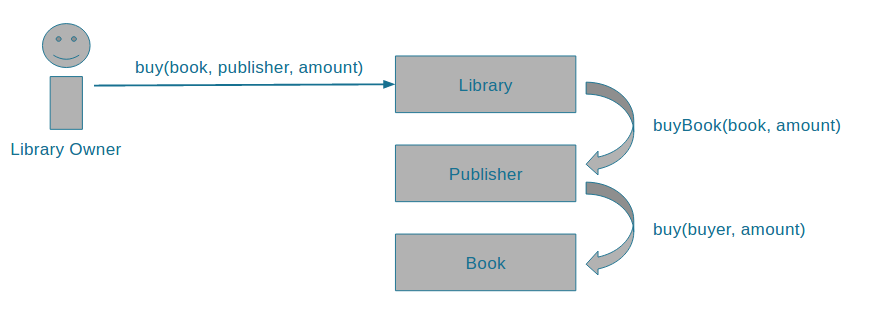
\includegraphics[width=\textwidth]{purchase.png}
%\begin{itemize}
%\item a library want's to buy some book instances
%\item calling the buy method on library contract
%\end{itemize}
\subsection{Book-Borrow}
To borrow a book, the user has to authenticate toward the library service on a classical way ( e.g. username/password). The library therefore knows, that the user is authorized to lend books. If the user wants to lend a book, he has to create a RSA-keypair. The private key is stored on the client site whereas the public key is submitted togehter with the book id to the library service.
Since the user is already authenticated, the library can forward this request to the library contract without any further verification.
The contract checks the availability of the requested book instances and stores the public key (see \ref{sssec:contractborrow}).

\vspace{0.3cm}
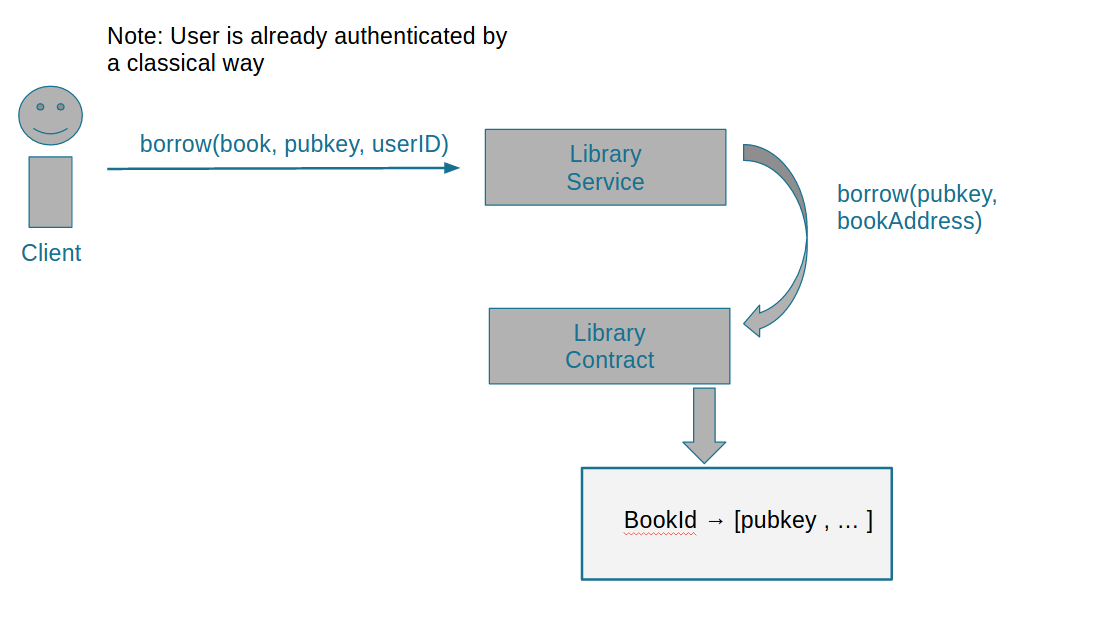
\includegraphics[width=\textwidth]{borrow.png}


\subsection{Access to digital media \label{sssec:access}}
If a user has borrowed a book, he can call the gateway-address that is stored in the book contract. That could be a normal internet address that routes the user to the publishers book service.
The user can now create a view request by submitting the publickey (which he has submitted to the library on the borrow request) and the book id that he encrypts with the appropriate private key.

By decrypting the book id with the submitted public key, the publisher can verify that the user is in possession of the private key. If this is successful, he can check that the public key is associated with a current loan of the book on the library. \imp{incomplete}


\vspace{0.3cm}
\includegraphics[width=\textwidth]{access.png}


\subsection{Book-Return}

\section{Metrics}

\section{How to implement a Publisher Service?}

